\documentclass[12pt]{article}
\usepackage[utf8]{inputenc}
\usepackage{amsmath}
\usepackage[T1]{fontenc}


\title{ECE 3413 Lab 04\\*Analysis of Linear Time Invariant (LTI) Systems}
\author{Leomar Dur\'an}
\date{${28}^{\text{th}}$ February 2023}

\usepackage{hyperref}

\usepackage[per-mode=symbol]{siunitx}
\newcommand*\siexpr[2][]{\SI[parse-numbers=false,#1]{#2}}%
\usepackage{xfrac}
\usepackage{amssymb}
\newcommand*\transpose{\mathsf{T}}

\usepackage{mathtools}%
\DeclarePairedDelimiter\brao()%
\DeclarePairedDelimiter\brac[]%
\DeclarePairedDelimiter\braco[)%
\DeclarePairedDelimiter\Brac\{\}%
\DeclarePairedDelimiter\norm\lVert\rVert%
\DeclarePairedDelimiter\piecefn\{.
\DeclarePairedDelimiter\evalat.|

\usepackage{lib/nonfloatenvirons}
\usepackage{booktabs}
\newcommand\ra[1]{\renewcommand*\arraystretch{#1}}
\ra{1.25}
\usepackage{minted}

\usepackage{adjustbox}
\newcommand*\mcadj[7]%
% {#columns}{col spec}{rotation}{adjust spec}
% {before rotated text}{rotated text}{after rotated text}
{%
    \multicolumn{#1}{#2}{%
        \rlap{%
            #5\adjustbox{rotate=#3,#4}{#6}~#7%
        }%
    }%
}

\usepackage{pdfpages}
\usepackage{standalone}
\usepackage{matlab}

\usepackage[skip=\baselineskip,indent=0pt]{parskip}
\setlength\parindent{0pt}

\def\hr{{\par\noindent\rule{\textwidth}{0.4pt}}}

\begin{document}

\maketitle
\newpage

\section{Introduction}

The purpose of this lab is to introduce the trace tools in Simulink that can be used in combination with the scope.
It also introduces the concept of file input and output of time series in Matlab and Simulink.
Generally, this experiment makes much more use of Simulink than we have so far.

Here we learn to expand on automating the process of finding transfer function characteristics from the step response that we have been working with in class.

\section{Procedure}

\subsection{Part 01 -- Standard signal responses}

\subsubsection{Step 01.01 -- The simulation}

\paragraph{The Parameters}

In part $1$ we are using standard input functions and applying the transfer function
$$
    G = \frac2{s^2 + 5 s + 9}
$$
to these.

I have written a Matlab script to parameterize the model so that it is more flexible and reusable.
This script is available in Appendix subsection \ref{sap:simulation params}.

It sets up the simulation time \mintinline{matlab}{TSTOP = 10.0} in \si\second, the parameters for the input function and the coefficients and constants for the transfer function.
In Part 01a, this input function is a step function which becomes \mintinline{matlab}{stepFinal = 1} in $\si\volt$ at time \mintinline{matlab}{Tstep = 0}.
In Part 01b, this input function is a ramp function $r(t)$ whose slope becomes $\SI1\volt$ at time \mintinline{matlab}{Tstep = 0} until $r(t) =$ \mintinline{matlab}{stepFinal = 1}.

This script is also reused in Part 02 since it already contains much of the input needed for part 02 (namely, the simulation time and transfer function.

\paragraph{01(a) The step response model}

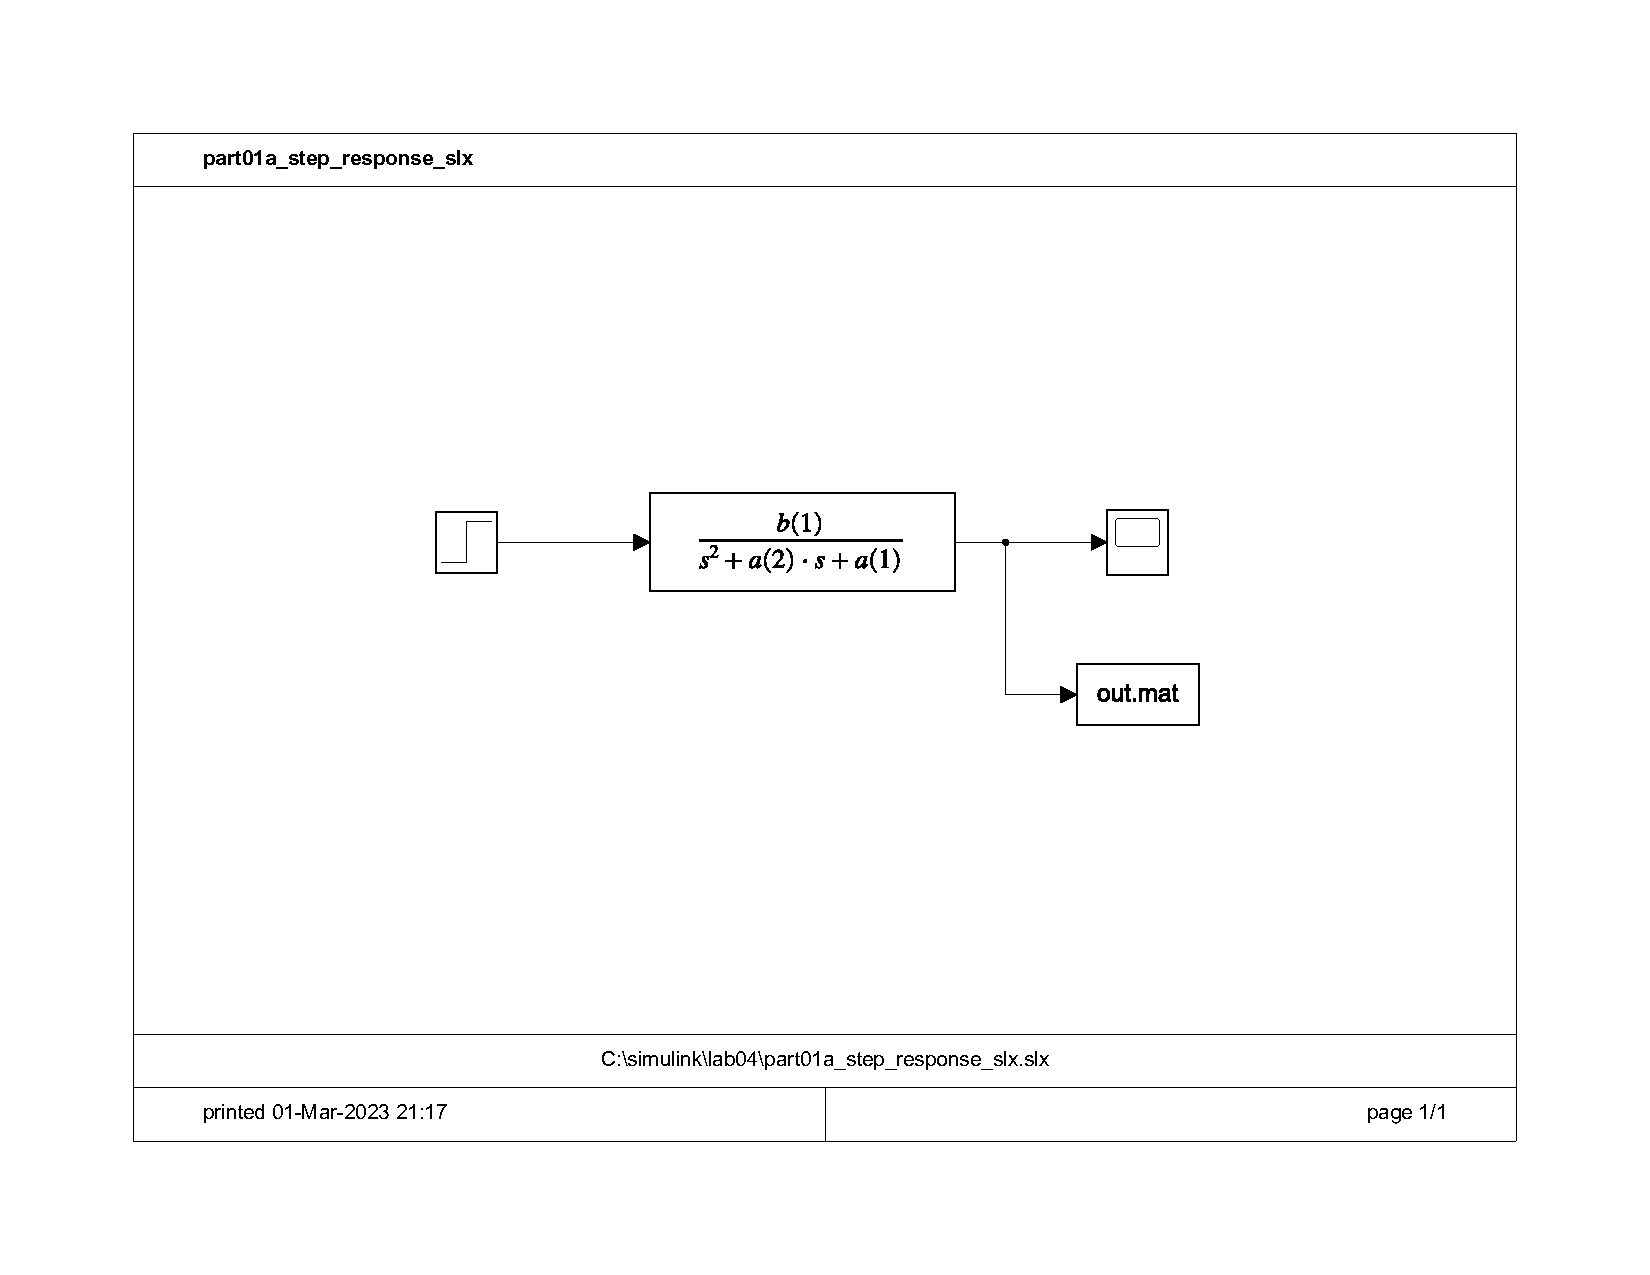
\includepdf[pages=1,landscape=true,pagecommand=\label{pdf:part01a}]{part01a_step_response_slx.pdf}

In Part 01(a), we are modeling a step response. Thus, our input signal is a Heaviside step function as built in
the model on page \pageref{pdf:part01a}.
% Fig. \ref{fig:step response model system}.
The only unique block in this model, the Step block is configured as in Fig. \ref{fig:step response model parameters}.

% \begin{figure}[h]
    % \centering
    % 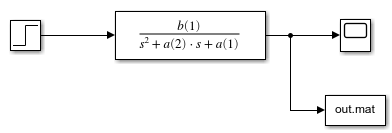
\includegraphics[width=\linewidth]{part01a_step_response_model.png}
    % \caption{The system over all for the step response.}
    % \label{fig:step response model system}
% \end{figure}

\begin{figure}[h]
    \centering
    % 689px = 5in
    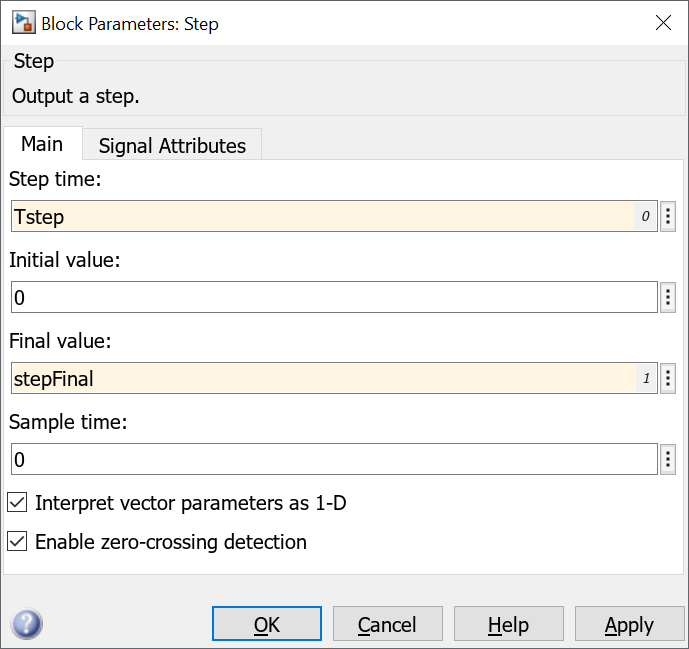
\includegraphics[width=(5in/689)*689]{part01a_step_parameters.png}
    \caption{The configuration for step.}
    \label{fig:step response model parameters}
\end{figure}

\paragraph{Common features}\label{par:common features}

The following features are common to all models simulated in this lab.
All parameters are defined in Appendix subsection \ref{sap:simulation params}.

\begin{figure}[h]
    \centering
    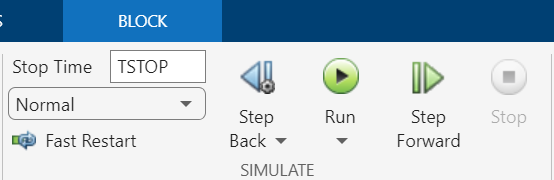
\includegraphics[width=(5in/689)*554]{common_simulation_time.png}
    \caption{The simulation time used in this equation is \mintinline{matlab}{TSTOP}.}
    \label{fig:common simulation time}
\end{figure}

\begin{figure}[h]
    \centering
    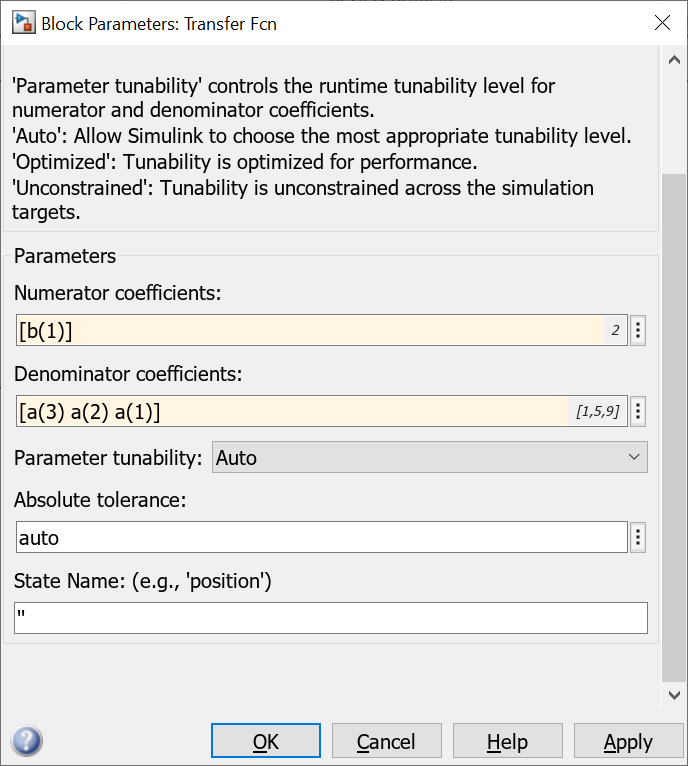
\includegraphics[width=(5in/689)*464]{common_transfer_fcn.png}
    \caption{The transfer function is $\frac{b_1}{s^2 + a_2 s + a_1}$. (Note that Matlab uses $1$-indexed arrays.)}
    \label{fig:common transfer fcn}
\end{figure}

\begin{figure}[h]
    \centering
    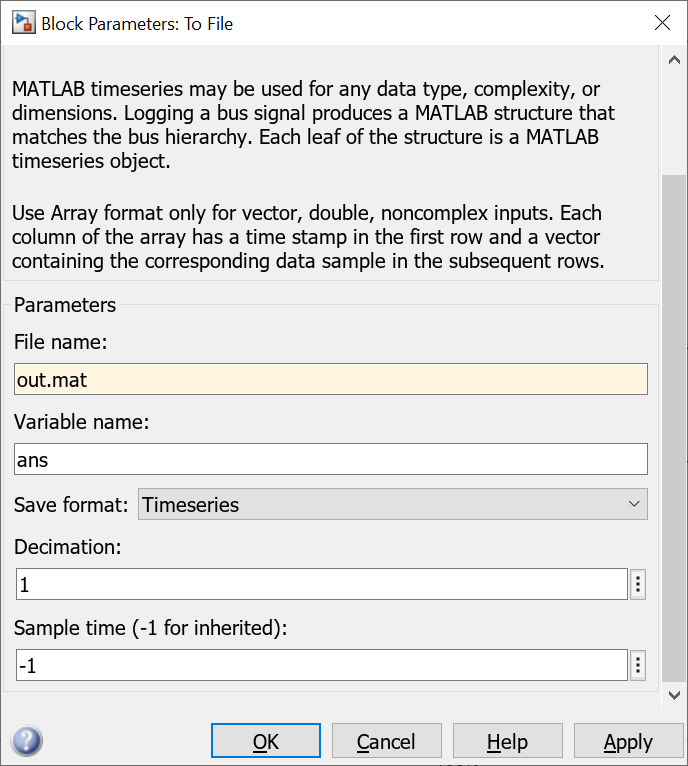
\includegraphics[width=(5in/689)*688]{common_to_file.png}
    \caption{All models will output the time series data of the response to the file \mintinline{matlab}{out.mat} to the default variable \mintinline{matlab}{ans}.}
    \label{fig:common to file}
\end{figure}

\paragraph{01(b) The ramp response model}

We use the same features described in paragraph \ref{par:common features}.
However, the difference is that we are modelling the ramp response seen
in the model on page \pageref{pdf:part01b}.
% in Fig. \ref{fig:ramp response model system}
with the ramp parameters in Fig. \ref{fig:ramp response model parameters}.

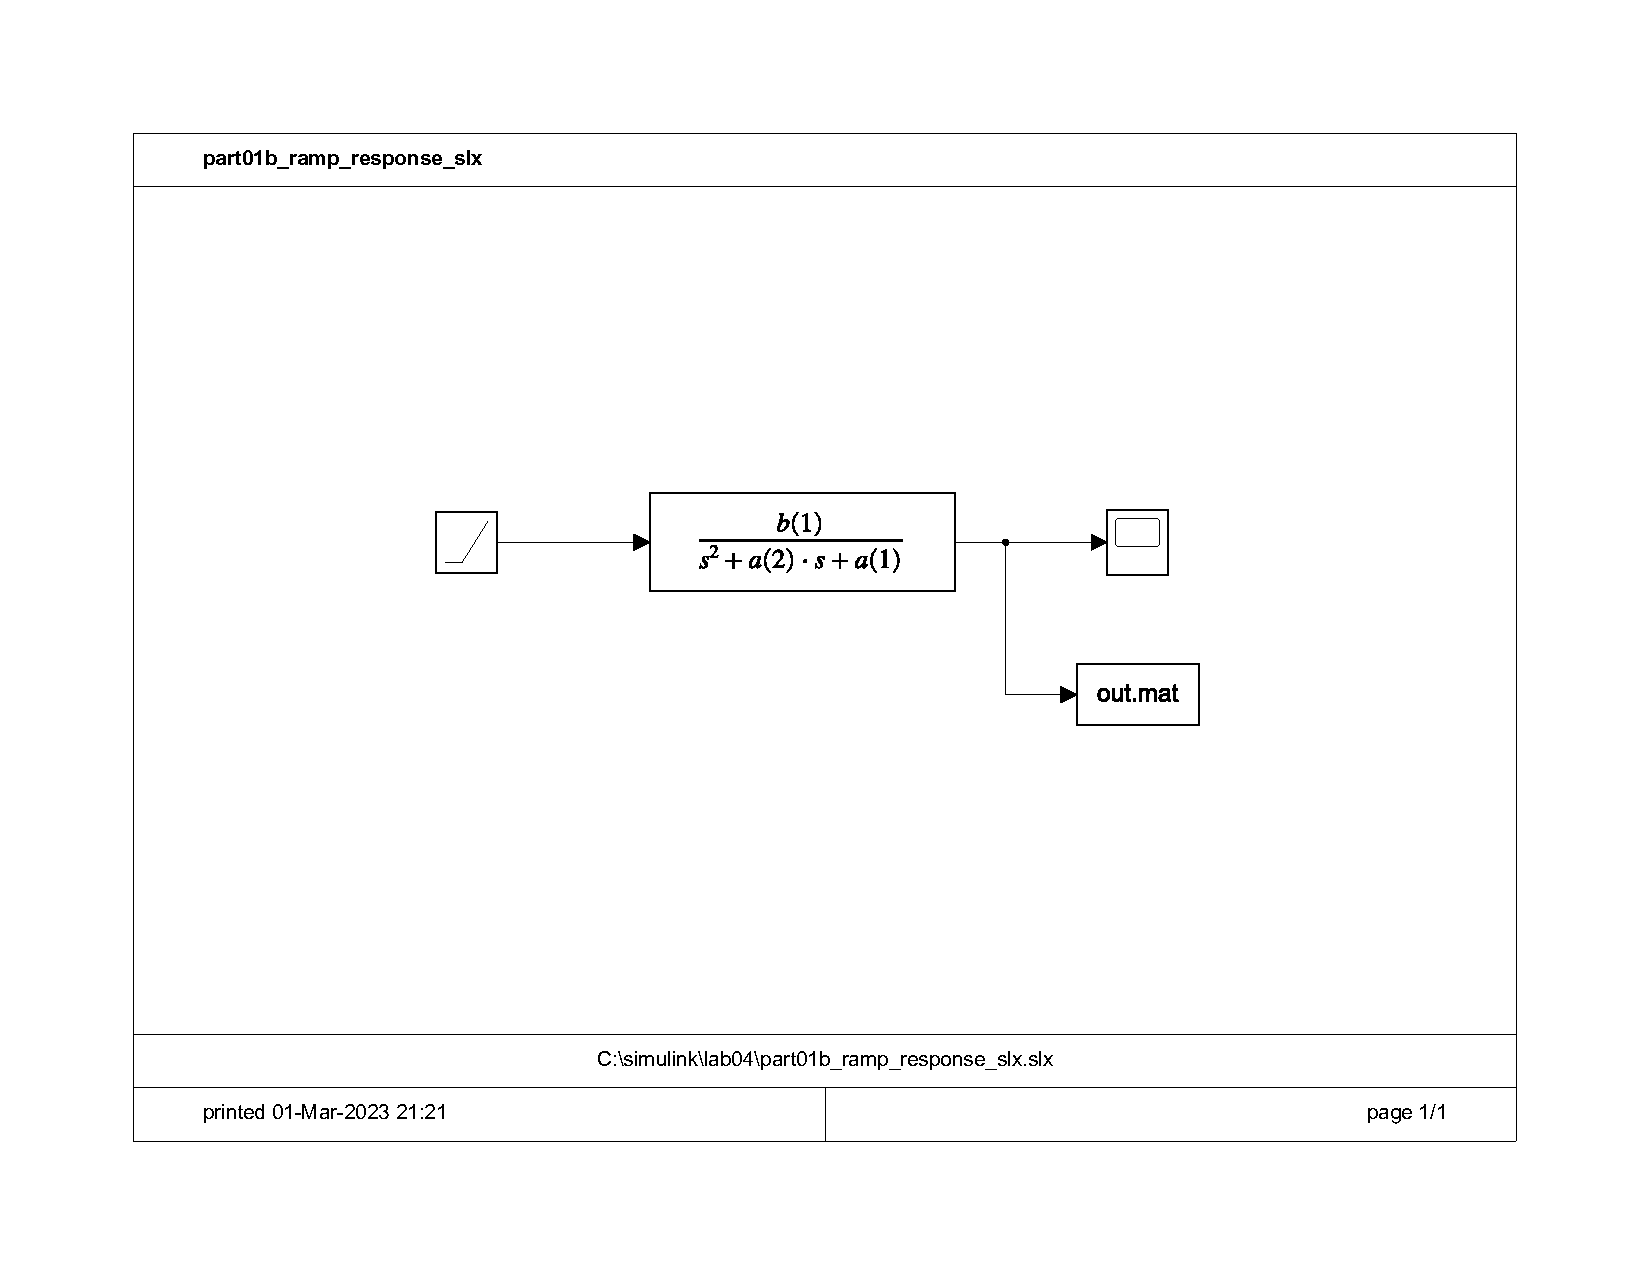
\includepdf[pages=1,landscape=true,pagecommand=\label{pdf:part01b}]{part01b_ramp_response_slx.pdf}

% \begin{figure}[h]
    % \centering
    % 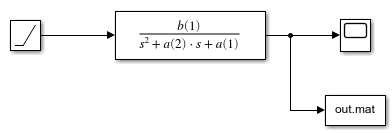
\includegraphics[width=\linewidth]{part01b_ramp_response_model.png}
    % \caption{The system over all for the ramp response.}
    % \label{fig:ramp response model system}
% \end{figure}

\begin{figure}[h]
    \centering
    % 689px = 5in
    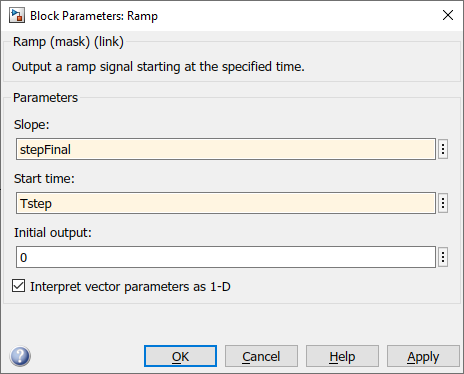
\includegraphics[width=(5in/689)*464]{part01b_ramp_parameters.png}
    \caption{The configuration for ramp.}
    \label{fig:ramp response model parameters}
\end{figure}

\subsubsection{Step 01.02 -- Measuring the traces on step response}

As before, we find the maximum

\paragraph{The peak} is found by finding the maximum output value of the plot.
We find the peak $c\brao{T_p} = \num{2.242e-1}$ in Fig. \ref{fig:step - measuring peak}.

\paragraph{The peak time} is the corresponding time, which we can find in the same plot.
The peak time $T_p \in \brac{{1.879}, {1.904}}\si\second$.
Let's take $T_p = \frac12\brao*{1.879 + 1.904}\si\second = \SI{1.8915}\second$.

\begin{figure}[h]
    \centering
    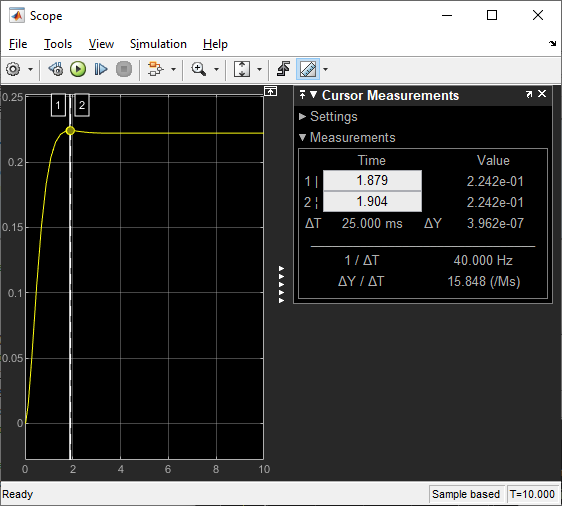
\includegraphics[width=\linewidth]{part01a_measuring_peak.png}
    \caption{Measuring the peak and peak time.}
    \label{fig:step - measuring peak}
\end{figure}

\paragraph{The percent overshoot} can be measured using Fig. \ref{fig:step - measuring percent overshoot}.
This is because cursor $1$ is at the peak time and cursor $2$ is on the final time.
So the percent overshoot is the value $\frac{\Delta Y}{c\brao{T_p}} = \frac{\num{1.929e-03}}{\num{2.242e-1}}\times\SI{100}\percent = \SI{0.8604}\percent$.
 
\begin{figure}[h]
    \centering
    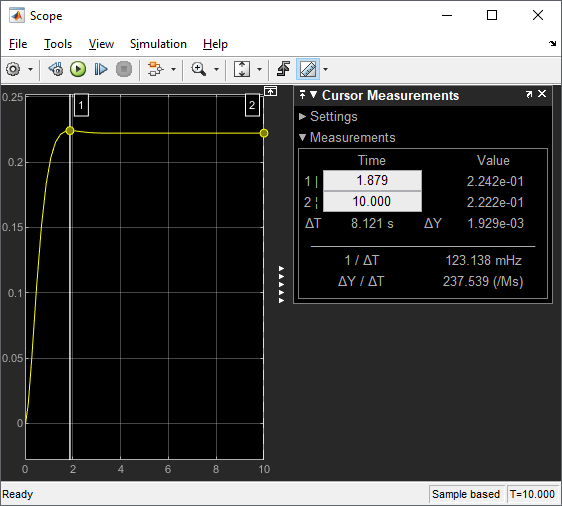
\includegraphics[width=\linewidth]{part01a_measuring_pcOS.png}
    \caption{Measuring the percent overshoot, final value and steady state error.}
    \label{fig:step - measuring percent overshoot}
\end{figure}

\paragraph{The stead state error}
We can also see the final value $c_f = \num{2.222e-1}$ in this figure,
and from that, we can calculate the steady state error.
We expect a final value equal to \mintinline{matlab}{stepFinal = 1}.
So $E_{ss} = 1 - \num{2.222e-1} = 0.7778$.

\paragraph{The rise time} To measure the rise time,
we must first find each of the first times when the output value is $\SI{10}\percent$ and $\SI{90}\percent$
of the final value.

\begin{figure}[h]
    \centering
    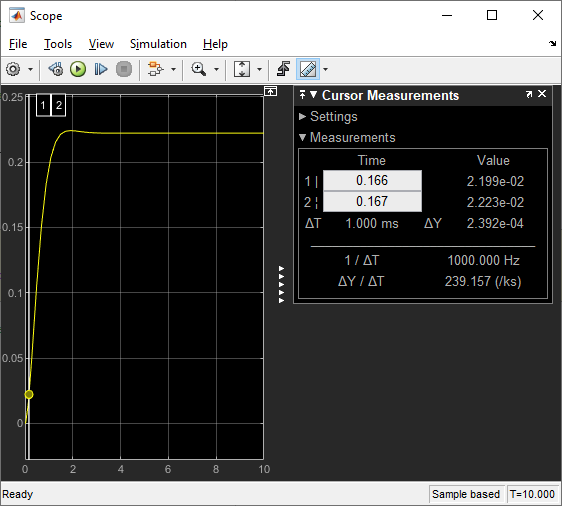
\includegraphics[width=\linewidth]{part01a_measuring_pc10.png}
    \caption{Estimating \SI{10}\percent of final output.}
    \label{fig:step - estimating 10 percent}
\end{figure}

Well, $\SI{10}\percent$ of the final value $\SI{10}\percent c_f = \SI{10}\percent \brao*{\num{2.222e-1}} = \num{2.222e-2}$.
In Fig. \ref{fig:step - estimating 10 percent}, we estimate the time when $c = \num{2.222e-2}$ to be
$$
	t_{.10} = \brao*{0.166 + \frac{\num{1e-3}}{\num{2.392e-02}}\brao*{\num{2.222e-2} - \num{2.199e-2}}}\si\second = \SI{0.16601}\second.
$$

\begin{figure}[h]
    \centering
    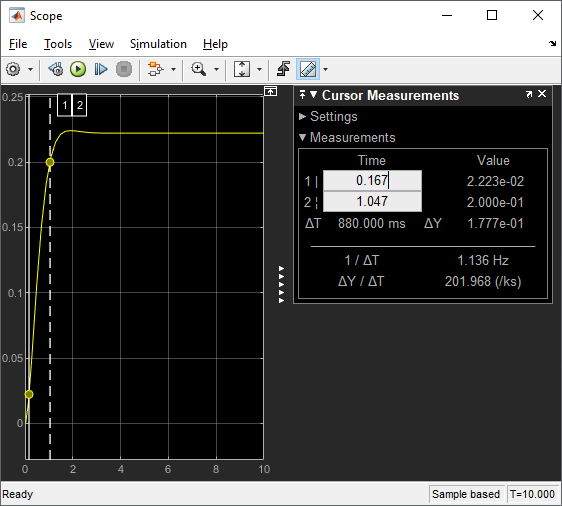
\includegraphics[width=\linewidth]{part01a_measuring_rise_time_estimate_+=.png}
    \caption{Measuring the rise time from $\SI{90}\percent$ and an estimate of $\SI{10}\percent$ of final output.}
    \label{fig:step - measuring rise time}
\end{figure}

Now $\SI{90}\percent$ of the final value $\SI{90}\percent c_f = 0.0200$.
In Fig. \ref{fig:step - measuring rise time}, we already have an exact measure of the time when $c = 0.0200$.
So let's just use that time $t_{.90} = 1.047$.
The time at cursor $1$ represents the closest time to $3$ decimal places.

The rise time $T_r = t_{.90} - t_{.10} = 1.047 - 0.16601 \si\second = \siexpr{0.88099}\second$.

\paragraph{The settling time} is when the output reaches a value within $\SI5\percent$ of its final value.
Now, the signal can never supersede the maximum value of the signal, the peak $c\brao{T_p} = \num{2.242e-1}$.

However, $c_f + \SI{5}\percent = \num{2.222e-2}\brao{1 + .05} + \num{2.333e-2}$.
So we look for the last value where $c = c_f - \SI{5}\percent = \num{2.111e-2}$.
From Fig. \ref{fig:step - measuring setting time}, we see that this occurs at $T_s = \SI{1.208}\second$.

\begin{figure}[h]
    \centering
    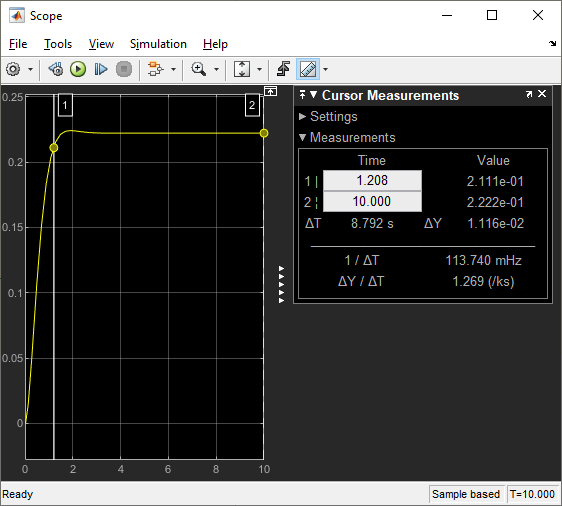
\includegraphics[width=\linewidth]{part01a_measuring_settling_time.png}
    \caption{Measuring the settling time.}
    \label{fig:step - measuring setting time}
\end{figure}

\subsubsection{Step 02 - Measuring the traces on ramp response}

% rise time
% 10%: 1.507
% 9.054 + 4.000e-3/8.889e-04 * (1.889e+0 - 1.8891)
% 9.049 + 5.000e-3/1.111e-03 * (1.8891 - 1.887e+0)
% 90%: 9.0585

% Peak, settling time
% 9.526 + 5.000e-3/1.111e-03 * (1.9941 - 1.993e+0)
% -5%: 9.5310

\paragraph{The peak} As before, we find the maximum output value of the plot.
We see in Fig. \ref{fig:ramp - measuring peak}, that the final value $c_f = \num{2.099e+0}$.

\paragraph{The peak time} The peak occurs at time $T_p = \SI{10.000}\second$.

\begin{figure}[h]
    \centering
    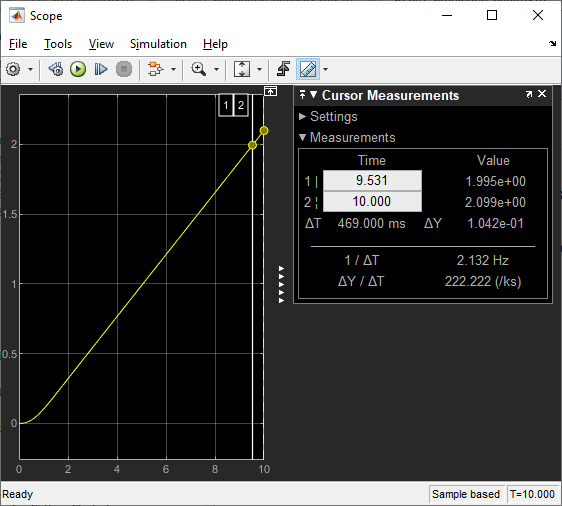
\includegraphics[width=\linewidth]{part01b_measuring_peak.png}
    \caption{Measuring the peak, peak time, the percent overshoot, final value, steady state error, and the settling time.}
    \label{fig:ramp - measuring peak}
\end{figure}

\paragraph{The percent overshoot}
In the case of the ramp response to the $G$, the maximum value is the final value.
Thus, the percent overshoot is $\frac{0}{2.099e+0} \times \SI{100}\percent = \SI{0.000}\percent$.

\paragraph{The stead state error} is $1 - c_f = 1 - \num{2.099e+0} = -1.0990$.

\paragraph{The rise time} is the time it takes for the signal to rise
from $\SI{10}\percent$, $t_{.10} = \SI{1.507}\second$
to $\SI{90}\percent$, $t_{.90} = \SI{9.0585}\second$,
that is $T_r = \SI{9.0585}\second - \SI{1.507}\second = \SI{7.5515}\second$.

\begin{figure}[h]
    \centering
    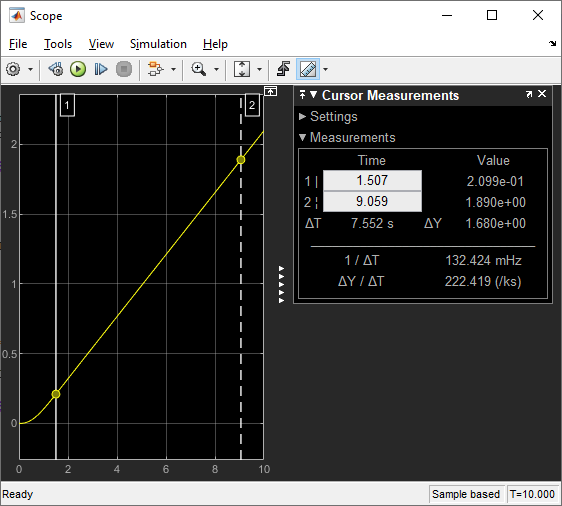
\includegraphics[width=\linewidth]{part01b_measuring_rise_time.png}
    \caption{Measuring the rise time from $\SI{90}\percent$ and an estimate of $\SI{10}\percent$ of final output.}
    \label{fig:ramp - measuring rise time}
\end{figure}

\paragraph{The settling time} can be see back in Fig. \ref{fig:ramp - measuring peak}.
The ramp response is within $\SI5\percent$ of the final value at time $T_s = \SI{9.5310}\second$.

\subsubsection{Step 01.03 -- Simulation analysis using Matlab}

To perform the analysis of the step and ramp response,
I have written the Matlab Live Script available in Appendix subsection \ref{sap:simulation analysis mlx}.

\subsection{Part 02 -- Writing in Matlab/Reading in Simulink}

We can write a signal in Matlab using a script such as that available in Appendix subsection \ref{sap:save sinusoid}
To analyze the effect of the transfer function on the generated sinusoidal function,
we use the model on page \pageref{pdf:part02}.

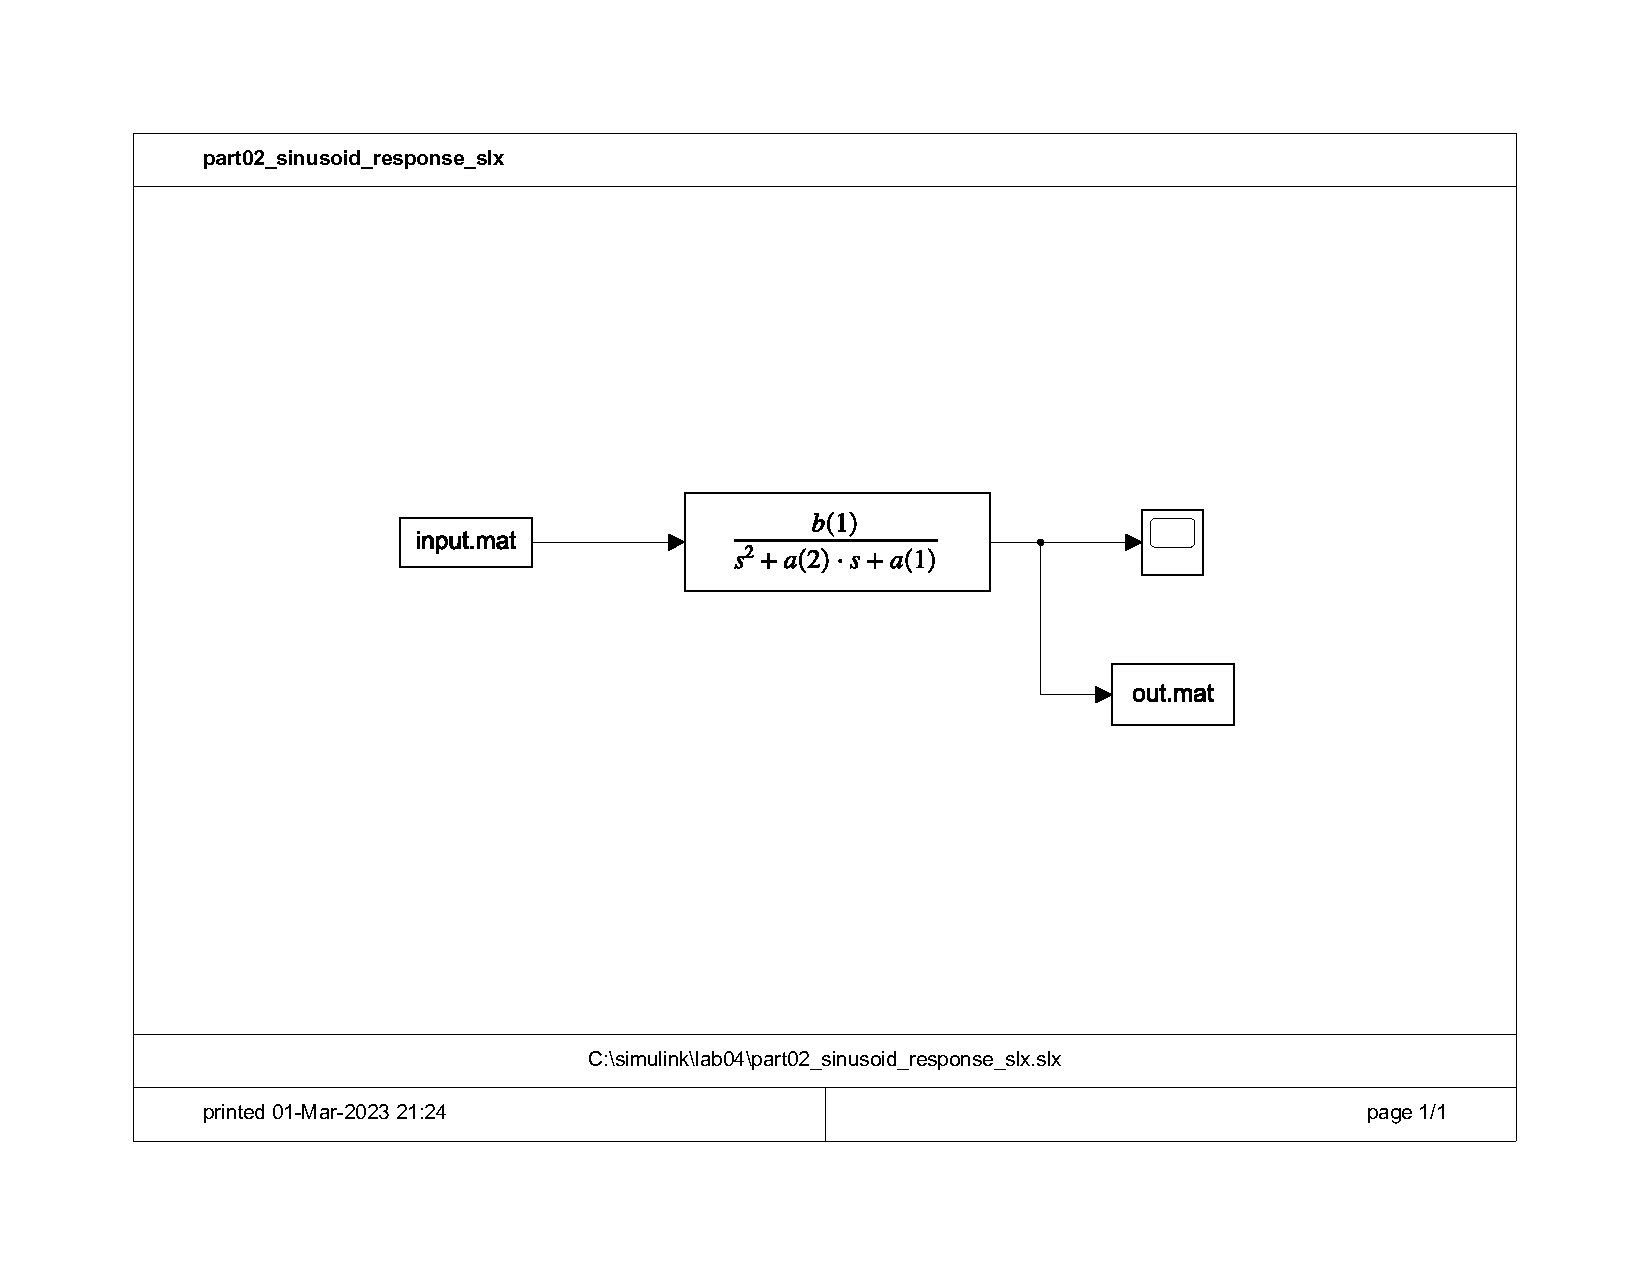
\includepdf[pages=1,landscape=true,pagecommand=\label{pdf:part02}]{part02_sinusoid_response_slx.pdf}

\section{Results}

\subsection{Part 01 -- Standard signal responses}

Following the procedure, we have found the values in Table \ref{tab:results of cursor calculation}.

\begin{table}[h]
    \centering
    \caption{The characteristics of the transfer function's responses calculated using traces.}
	\[
		\begin{array}{@{}l*7S@{}}
		\toprule
			\text{Response} & T_p \brac{\si\second} & c\brao{T_p} & \si\percent OS & \text{$E_{ss}$} & T_r \brac{\si\second} & T_s \brac{\si\second}
		\\*
		\midrule
			\text{Step} & 1.8915 & 0.2242 & \SI{0.8604}\percent & 0.7778 & 0.88099 & 1.208
		\\*
			\text{Ramp} & 10.000 & 2.099 & \SI{0.000}\percent & -1.0990 & 7.5515 & 9.5310
		\\*
		\bottomrule
		\end{array}
	\]
    \label{tab:results of cursor calculation}
\end{table}

\subsubsection{Step 03 -- Analyses by Matlab}

Here we see the results of the analyses by Matlab using the Matlab live script.
We compare to the values that we found by using the traces using the percent difference formula

\begin{equation}
	\text{$\si\percent$ difference} = \frac{\Delta x}{\bar{x}}\times\SI{100}\percent
\end{equation}

% This LaTeX was auto-generated from MATLAB code.
% To make changes, update the MATLAB code and export to LaTeX again.

\documentclass{article}

\usepackage[utf8]{inputenc}
\usepackage[T1]{fontenc}
\usepackage{lmodern}
\usepackage{graphicx}
\usepackage{color}
\usepackage{hyperref}
\usepackage{amsmath}
\usepackage{amsfonts}
\usepackage{epstopdf}
\usepackage[table]{xcolor}
\usepackage{matlab}

\sloppy
\epstopdfsetup{outdir=./}
\graphicspath{ {./part01a_step03_simulation_analysis_mlx_images/} }

\begin{document}

\matlabtitle{Simulation analysis $-$ Step response}


\matlabheading{Read the data file and load its data}

\begin{matlaboutput}
TSTOP = 10
\end{matlaboutput}
\begin{matlaboutput}
Tstep = 0
\end{matlaboutput}
\begin{matlaboutput}
stepFinal = 1
\end{matlaboutput}
\begin{matlaboutput}
data = 
    ans: [1x1 timeseries]

\end{matlaboutput}

\matlabheading{Part 01-03 perform step analysis}

\begin{par}
\begin{flushleft}
We calculate the analysis using these intermediate values.
\end{flushleft}
\end{par}

\begin{matlaboutput}
pc10Idx = 8
\end{matlaboutput}
\begin{matlaboutput}
pc90Idx = 12
\end{matlaboutput}
\begin{matlaboutput}
TsIdx = 12
\end{matlaboutput}

\begin{par}
\begin{flushleft}
The results are
\end{flushleft}
\end{par}

\begin{matlaboutput}
stepCharacteristics = 
    peak: 0.2242
    pcOS: 0.8771
      Tr: 0.7997
      Tp: 1.8865
      Ts: 1.0865
     Ess: 0.7778

\end{matlaboutput}

\begin{par}
\begin{flushleft}
Plot the steady state error, followed by the plot with characteristics traced.
\end{flushleft}
\end{par}

\begin{center}
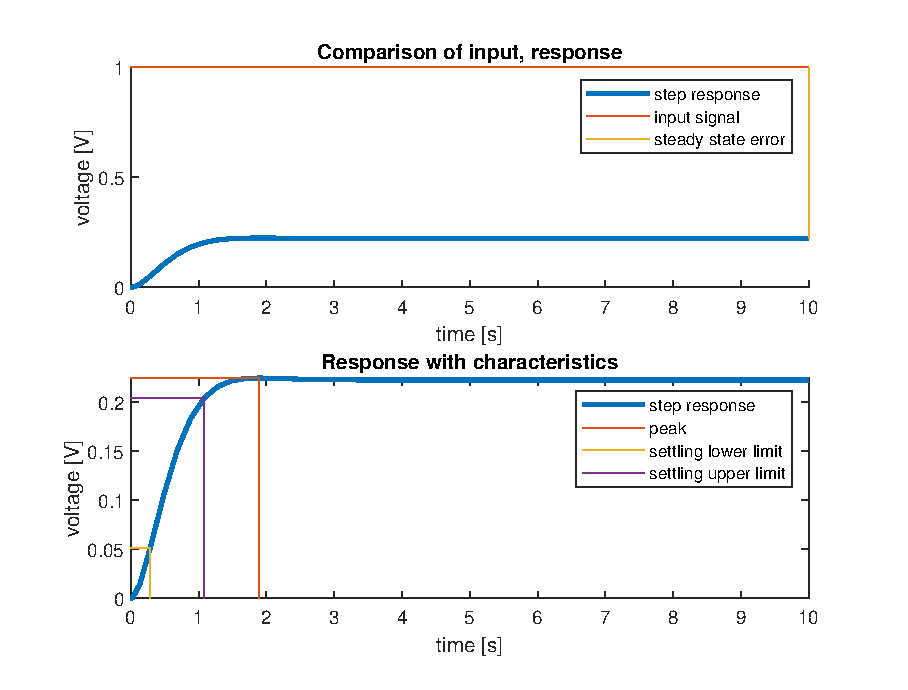
\includegraphics[width=\maxwidth{56.196688409433015em}]{figure_0.eps}
\end{center}
\end{document}


\begin{table}[h]
    \centering
    \caption{Comparison of step responses: by traces and by Matlab.}
	\[
		\begin{array}{@{}l*7S@{}}
		\toprule
			\text{Analysis} & T_p \brac{\si\second} & c\brao{T_p} & \si\percent OS & \text{$E_{ss}$} & T_r \brac{\si\second} & T_s \brac{\si\second}
		\\*
		\midrule
			\text{Trace} & 1.8915 & 0.2242 & \SI{0.8604}\percent & 0.7778 & 0.88099 & 1.208
		\\*
			\text{Matlab} & 1.8865 & 0.2242 & \SI{0.8771}\percent & 0.7778 & 0.7997 & 1.0865
		\\*
		\midrule
			\text{$\si\percent$ difference} & \SI{0.2647}\percent & \SI{0.0000}\percent & \SI{1.9223}\percent & \SI{0.0000}\percent & \SI{9.6734}\percent & \SI{10.5905}\percent
		\\*
		\bottomrule
		\end{array}
	\]
    \label{tab:comparison of step response analyses}
\end{table}

% This LaTeX was auto-generated from MATLAB code.
% To make changes, update the MATLAB code and export to LaTeX again.

\documentclass{article}

\usepackage[utf8]{inputenc}
\usepackage[T1]{fontenc}
\usepackage{lmodern}
\usepackage{graphicx}
\usepackage{color}
\usepackage{hyperref}
\usepackage{amsmath}
\usepackage{amsfonts}
\usepackage{epstopdf}
\usepackage[table]{xcolor}
\usepackage{matlab}

\sloppy
\epstopdfsetup{outdir=./}

\begin{document}

\matlabtitle{Simulation analysis $-$ Ramp response}


\matlabheading{Read the data file and load its data}

\begin{matlaboutput}
TSTOP = 10
\end{matlaboutput}
\begin{matlaboutput}
Tstep = 0
\end{matlaboutput}
\begin{matlaboutput}
stepFinal = 1
\end{matlaboutput}
\begin{matlaboutput}
data = 
    ans: [1x1 timeseries]

\end{matlaboutput}

\matlabheading{Part 01-03 perform step analysis}

\begin{par}
\begin{flushleft}
We calculate the analysis using these intermediate values.
\end{flushleft}
\end{par}

\begin{matlaboutput}
pc10Idx = 11
\end{matlaboutput}
\begin{matlaboutput}
pc90Idx = 49
\end{matlaboutput}
\begin{matlaboutput}
TsIdx = 50
\end{matlaboutput}

\begin{par}
\begin{flushleft}
The results are
\end{flushleft}
\end{par}

\begin{matlaboutput}
stepCharacteristics = 
    peak: 2.0988
    pcOS: 0
      Tr: 7.6000
      Tp: 10
      Ts: 9.3571
     Ess: -1.0988

\end{matlaboutput}

\begin{par}
\begin{flushleft}
Plot the steady state error, followed by the plot with characteristics traced.
\end{flushleft}
\end{par}

\begin{center}
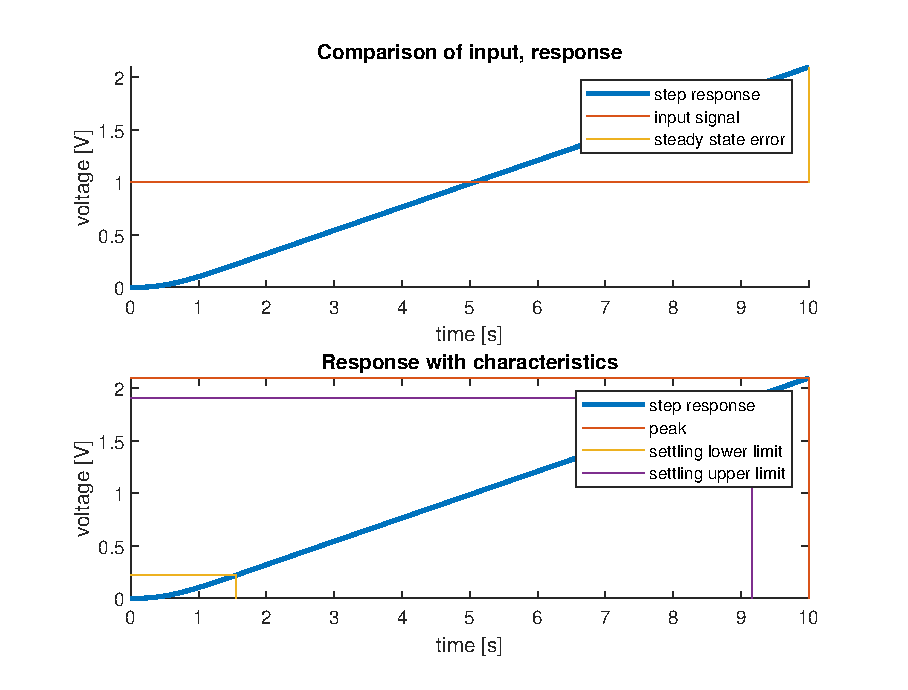
\includegraphics[width=\maxwidth{56.196688409433015em}]{./part01b_step03_simulation_analysis_mlx_images/figure_0.eps}
\end{center}
\end{document}


\begin{table}[h]
    \centering
    \caption{Comparison of ramp responses: by traces and by Matlab.}
	\[
		\begin{array}{@{}l*7S@{}}
		\toprule
			\text{Analysis} & T_p \brac{\si\second} & c\brao{T_p} & \si\percent OS & \text{$E_{ss}$} & T_r \brac{\si\second} & T_s \brac{\si\second}
		\\*
		\midrule
			\text{Trace} & 10.000 & 2.099 & \SI{0.000}\percent & -1.0990 & 7.5515 & 9.5310
		\\*
			\text{Matlab} & 10 & 2.0988 & \SI{0}\percent &  -1.0988 & 7.6000 & 9.3571
		\\*
		\midrule
			\text{$\si\percent$ difference} & \SI{0.}\percent & \SI{9.5288e-03}\percent & \SI{0.}\percent & \SI{1.8200e-02}\percent & \SI{0.6402}\percent & \SI{1.8414}\percent
		\\*
		\bottomrule
		\end{array}
	\]
    \label{tab:comparison of ramp response analyses}
\end{table}

Finally, let's compare the two methods by inspection.

\begin{table}[h]
    \centering
    \caption{Comparison of percent differences between step response and ramp response.}
	\[
		\begin{array}{@{}l*7S@{}}
		\toprule
			\text{Response} & T_p \brac{\si\second} & c\brao{T_p} & \si\percent OS & \text{$E_{ss}$} & T_r \brac{\si\second} & T_s \brac{\si\second}
		\\*
		\midrule
			\text{Step} & \SI{0.2647}\percent & \SI{0.0000}\percent & \SI{1.9223}\percent & \SI{0.0000}\percent & \SI{9.6734}\percent & \SI{10.5905}\percent
        \\*
			\text{Ramp} & \SI{0.}\percent & \SI{9.5288e-03}\percent & \SI{0.}\percent & \SI{1.8200e-02}\percent & \SI{0.6402}\percent & \SI{1.8414}\percent
		\\*
		\bottomrule
		\end{array}
	\]
    \label{tab:comparison of methods}
\end{table}

Looking at Table \ref{tab:comparison of methods},
although the percentage differences are not bad because we are estimating using a cursor, which leaves room for human error,
I am surprised to see that the ramp analysis is much closer and acceptable.
The settling time seems to be the hardest characteristic to approximate by using traces giving $\SI{1.8414}\percent$ even for the ramp response.

\subsection{Part 02 -- Writing in Matlab/Reading in Simulink}\label{ssc: I/O using matlab and simulink}

For this part of the experiment, we wrote a sinusoidal wave to a file using Matlab and read it as an input signal for a Simulink model.
My expectation is that since the sinusoidal wave is an oscillating signal with an indeterminate limit as time approaches infinity, that we will get an unstable output that oscillates and has an indeterminate limit as time approaches infinity.

\begin{figure}[h]
    \centering
    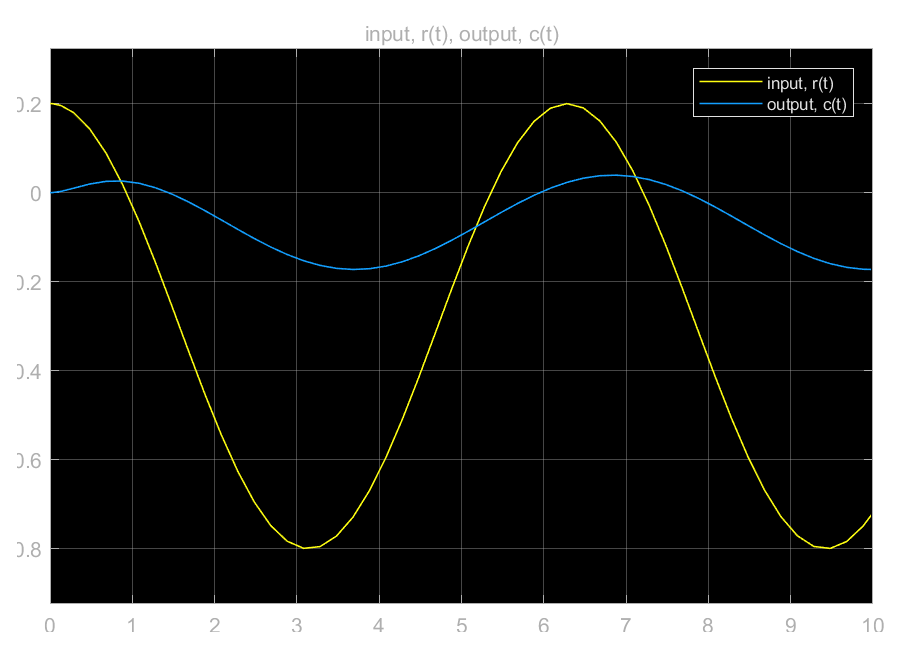
\includegraphics[width=\linewidth]{part02_scope.eps}
    \caption{Comparison of the input signal and the output signal from performing the transfer function thereon.}
    \label{fig:part02_scope}
\end{figure}

From Fig. \ref{fig:part02_scope}, we see that we do indeed get an oscillating output signal, which is very similar to a sine wave.

% This LaTeX was auto-generated from MATLAB code.
% To make changes, update the MATLAB code and export to LaTeX again.

\documentclass{article}

\usepackage[utf8]{inputenc}
\usepackage[T1]{fontenc}
\usepackage{lmodern}
\usepackage{graphicx}
\usepackage{color}
\usepackage{hyperref}
\usepackage{amsmath}
\usepackage{amsfonts}
\usepackage{epstopdf}
\usepackage[table]{xcolor}
\usepackage{matlab}

\sloppy
\epstopdfsetup{outdir=./}

\begin{document}

\matlabtitle{Simulation analysis $-$ Response to Sinusoidal from file}


\matlabheading{Read the data file and load its data}

\begin{matlaboutput}
TSTOP = 10
\end{matlaboutput}
\begin{matlaboutput}
Tstep = 0
\end{matlaboutput}
\begin{matlaboutput}
stepFinal = 1
\end{matlaboutput}
\begin{matlaboutput}
data = 
    ans: [1x1 timeseries]

\end{matlaboutput}

\matlabheading{Part 01-03 perform step analysis}

\begin{par}
\begin{flushleft}
We calculate the analysis using these intermediate values.
\end{flushleft}
\end{par}

\begin{matlaboutput}
pc10Idx = 1
\end{matlaboutput}
\begin{matlaboutput}
pc90Idx = 1
\end{matlaboutput}
\begin{matlaboutput}
TsIdx = 55
\end{matlaboutput}

\begin{par}
\begin{flushleft}
The results are
\end{flushleft}
\end{par}

\begin{matlaboutput}
stepCharacteristics = 
    peak: 0.0393
    pcOS: -122.7348
      Tr: 0
      Tp: 6.8808
      Ts: 10
     Ess: 1.1727

\end{matlaboutput}

\begin{par}
\begin{flushleft}
Plot the steady state error, followed by the plot with characteristics traced.
\end{flushleft}
\end{par}

\begin{center}
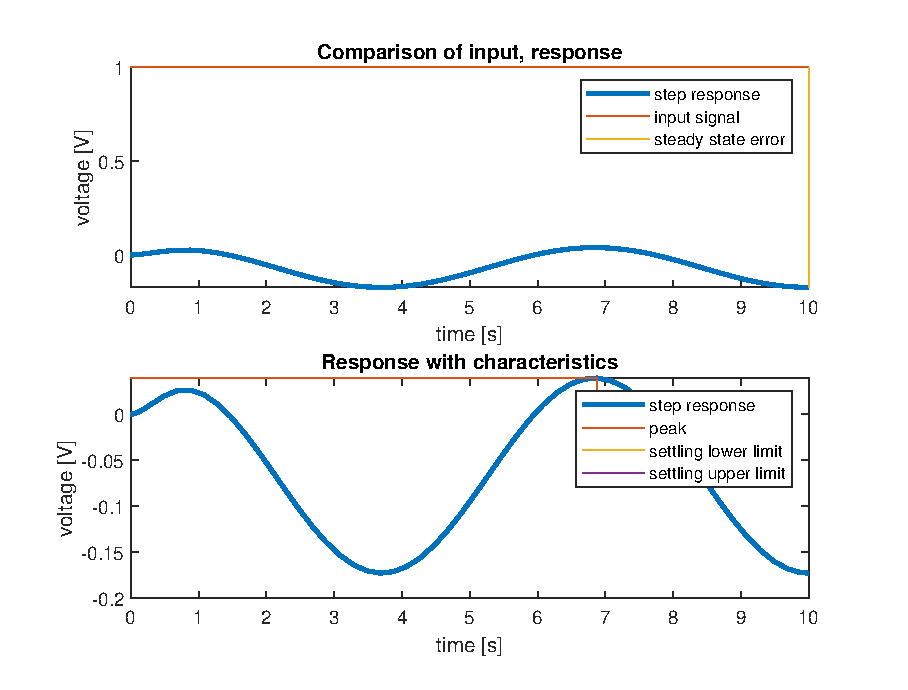
\includegraphics[width=\maxwidth{56.196688409433015em}]{./part02_step03_simulation_analysis_mlx_images/figure_0.eps}
\end{center}
\end{document}


In the preceding Matlab live script,
we saw that
the Simulation analysis script (Appendix subsection \ref{sap:simulation analysis mlx})
attempted to find all of the characteristics of the sinusoidal response.

In this case, the peak was exactly as expected (the maximum value).
Peak time refered to the corresponding first time that the sinusoidal response reached its maximum
during the time of the simulation.

However, the values of the percent overshoot, the rising time and steady state error made no sense because there is no final value to the signal.
This is because the limit of a sinusoidal function as time approaches infinite is indeterminate.

We can see that the settling time is near or at the entire time of the simulation because the sinusoidal response will never settle.

\section{Discussion}

This experiment showed that the process of finding a signal's characteristics through using the trace function can be found satisfactorily. It would also lead to less human error.

This experiment shows that the settling time may not be a good characteristic to use to identify a transfer function.

The characteristics that we found using the ramp response in Table \ref{tab:results of cursor calculation} were very different from those we found using step response. I am not completely sure how the ramp response would be used. Overall, the step response seems to be the best one to use to identify a transfer function as compared to both the ramp response and the sinusoidal as seen in subsection \ref{ssc: I/O using matlab and simulink}.

Finally, we can predict the oscillatory nature of an output signal by knowing whether any of its components also oscillate.

\newpage
\appendix
\section{Appendix}

\subsection{Step 01 (in parts 01 and 02) -- Simulation parameters, Matlab Script}\label{sap:simulation params}
\inputminted{matlab}{step01_simulation_params.m}

\hr

\subsection{Part 01 Step 03 -- Simulation analysis, Matlab Live Script}\label{sap:simulation analysis mlx}
\inputminted{matlab}{step03_simulation_analysis_mlx.m}

\hr

\subsection{Part 02 -- Saving a sinusoidal function, Matlab function}\label{sap:save sinusoid}
\inputminted{matlab}{part02_save_sinusoid.m}

\end{document}
